% vim: set textwidth=78 autoindent:

\section{Kern-Plugins verwenden}\label{sec:core_plugins}\index{plugins!core}

% when the revision of a section has been finalized, 
% comment out the following line:
%\updatedisclaimer

QGIS stellt 17 Kern-Plugins zur Verf�gung, die mit dem Plugin Manager geladen
und entladen werden k�nnen. In Tabelle~\ref{tab:core_plugins} finden Sie eine
Liste der Plugins mit dem jeweiligen Icon, �ber das Sie es in der
Werkzeugleiste aufrufen k�nnen und einer kurzen Beschreibung der
Funktionalit�t.\footnote{Die Plugins MapServer Export und
Plugin Installer sind externe Python Plugins, aber sie sind zugleich Teil des
QGIS Quellcodes und stehen daher automatisch wie ein Kern-Plugin im Plugin
Manager zur Verf�gung.}

% minipage is needed to appear the footnote under the table
% SH
\begin{minipage}{\textwidth}
\begin{table}[H]
\centering
\caption{QGIS Kern-Plugins}\label{tab:core_plugins}\medskip
\small
 \begin{tabular}{|l|l|p{4in}|}
\hline \textbf{Icon} & \textbf{Plugin} & \textbf{Beschreibung}\\
\hline

\includegraphics[width=0.6cm]{delimited_text}
 & Layer aus Textdatei laden \index{plugins!delimited text} & CSV-Tabellen mit X- und Y-Koordinaten darstellen\\
\hline

\includegraphics[width=0.6cm]{coordinate_capture}
 & Koordinaten abgreifen \index{plugins!coordinate capture}& Koordinaten in
anderem KBS aus dem Kartenfenster abgreifen\\
\hline 
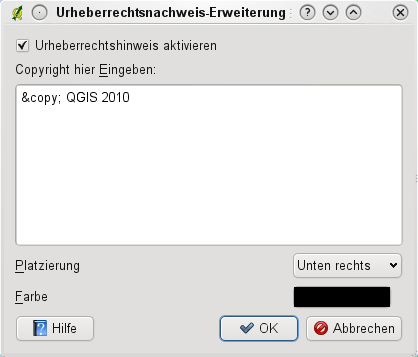
\includegraphics[width=0.6cm]{copyright_label}
 & Copyright Label \index{plugins!copyright}& Stellt
Urheberrechtsinformationen dar\\
\hline 

\includegraphics[width=0.6cm]{dxf2shp_converter}
 & DXF2Shape Konverter \index{plugins!DXF2Shape}& Wandelt Daten vom DXF ins
Shapefile Format um\\
\hline

\includegraphics[width=0.6cm]{gps_importer}
 & GPS Werkzeuge \index{plugins!gps}& Werkzeuge zum Laden und Importieren von
GPS-Daten\\
\hline

\includegraphics[width=0.6cm]{grass}
 & GRASS \index{plugin!grass toolbox} & GRASS-Layer einer Location anzeigen
und bearbeiten\\
\hline
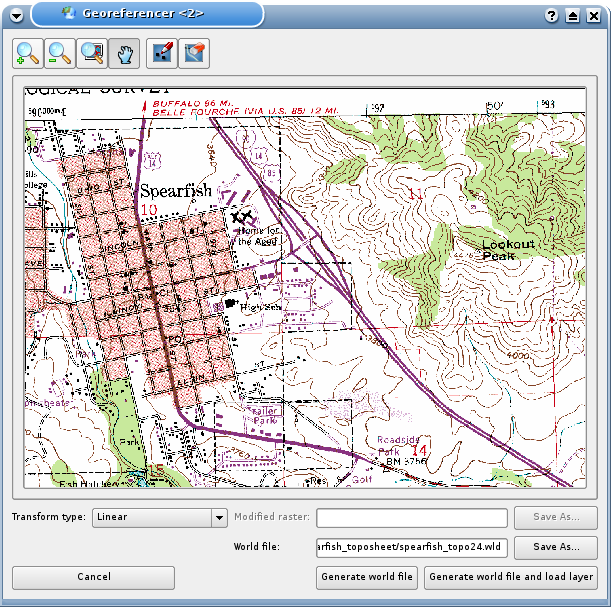
\includegraphics[width=0.6cm]{georeferencer}
 & Georeferenzierer \index{plugin!georeferencer} & F�gt
Projektionsinformationen zu einer Rasterdatei hinzu\\
\hline

\includegraphics[width=0.6cm]{grid_maker}
 & Gradnetz Generator \index{plugins!graticule}& Erstellt ein Gradnetz als
Lat/Lon und speichert es als Shapefile\\
\hline

\includegraphics[width=0.6cm]{interpolation}
& Interpolationsplugin \index{plugins!Interpolation}& Interpolation von
St�tzpunkten eines Vektorlayers in ein Raster\\
\hline

\includegraphics[width=0.6cm]{mapserver_export}
& MapServer Export \index{plugins!MapServer Export}& Exportiert eine QGIS
Projektdatei in einen MapServer Mapfile \\
\hline
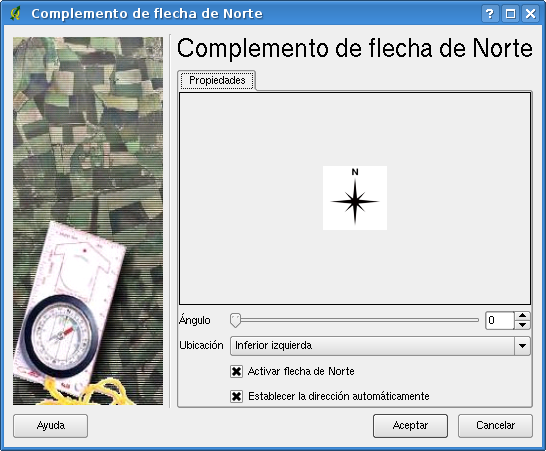
\includegraphics[width=0.6cm]{north_arrow}
& Nordpfeil \index{plugins!north arrow}& Stellt einen Nordpfeil im
Kartenfenster dar\\
\hline

\includegraphics[width=0.6cm]{ogr_converter}
 & OGR-Layer-Konverter \index{plugins!OGR converter} & Wandelt Vektorlayer
von einem OGR-unterst�tzten Vektorformat in ein anderes um\\
\hline

\includegraphics[width=0.6cm]{plugin_installer}
 & Plugin Installer \index{plugins!Plugin Installer} & Herunterladen und
installieren externer QGIS Python Plugins\\
\hline

\includegraphics[width=0.6cm]{spiticon}
 & SPIT \index{plugins!spit}& Importieren von Shapefiles nach PostGIS \\
\hline

\includegraphics[width=0.6cm]{quick_print}
 & Schnelles drucken \index{plugins!quick print}& Ohne gro�en Aufwand eine
einfache Karte drucken \\
\hline
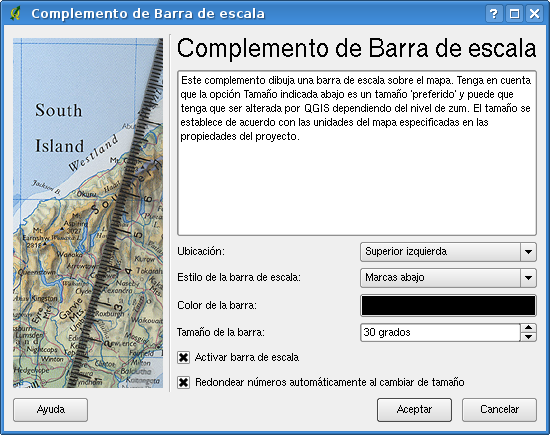
\includegraphics[width=0.6cm]{scale_bar}
 & Ma�stab \index{plugins!scalebar}& Zeichnet einen Ma�stab ins Kartenfenster\\
\hline

\includegraphics[width=0.6cm]{mIconAddWfsLayer}
 & WFS-Plugin & L�dt und stellt WFS-Layer dar \\
\hline
\end{tabular}
\end{table}
\end{minipage}

\normalsize

\begin{Tip}\caption{\textsc{Plugin Einstellungen als Projekt speichern}}\index{plugins settings}
\qgistip{Wenn Sie ein .qgs Projekt erstellen, werden alles Einstellungen
bez�glich des Nordpfeil, Ma�stab und Copyright Plugins mitgespeichert und
beim n�chsten Laden des Projektes wieder dargestellt.}
\end{Tip}

